\chapter{The nEDM active magnetic shielding}

\label{ch:nedm_sfc}


\section{Introduction}
\cite{Franke2013}

\subsection{Motivation}

\subsection{The nEDM SFC system}

\subsection{SFC matrix}
\begin{figure}[bth]
  \myfloatalign
  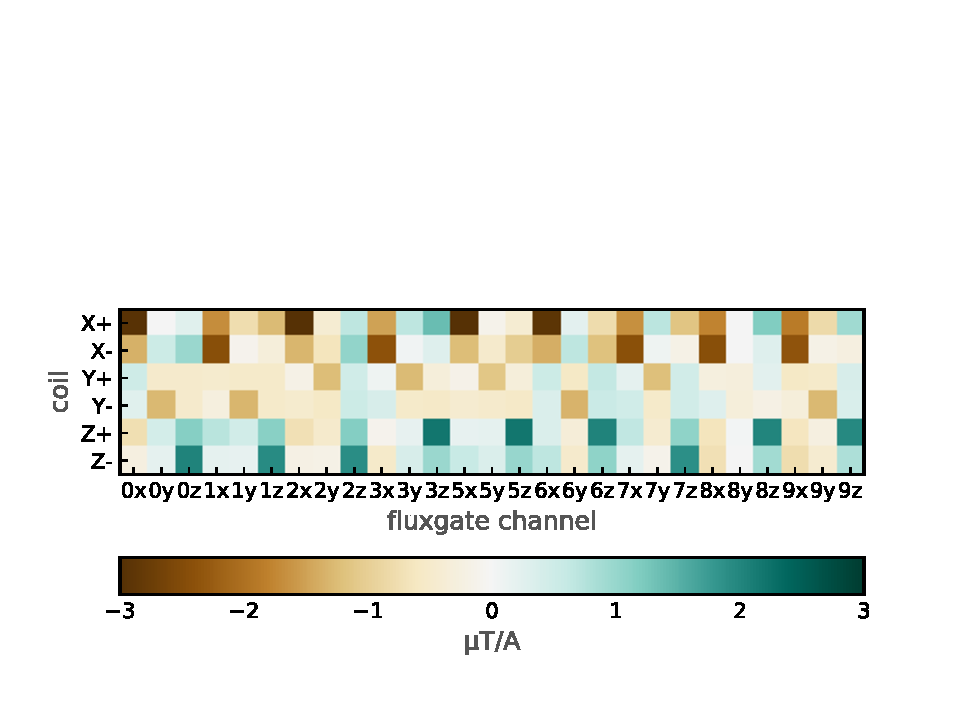
\includegraphics[width=.8\linewidth]{gfx/nEDM_SFC/nEDM_SFC_matrix}
  \caption
  [TODO]
  {The SFC matrix measured by Franke on 2012-11-07 (see \cite{Franke2013}) in the thermohouse coordinates.}
  \label{fig:nEDM_SFC_matrix}
\end{figure}

\subsection{Fluxgates}

\section{Influence of the SC magnet}


\section{Magnetic field during sparks in HV}


\section{Possible mistake in implementation}
Need to provide screenshots of the codehere.

Work of Nick Schwegler.


\section{The spectrum of the SFC matrix}
The SFC matrix used during the data taking of the nEDM experiment (2014, 15 and 16) is the one measured by Franke \cite{Franke2013}. The matrix not only needed to be inverted, but also additionally regularised. While it has been thoroughly discussed how to do the regularisation, the question of why was it needed at all was neither posed nor answered.

Let us elaborate on regularisation. The SFC matrix represents coefficients in a set of linear equations that need to be solved in order to determine the best currents to apply for a given goal field. As the set of equation is over--determined, the best solution is found by the least--squares, which is exactly equivalent to calculating the pseudoinverse matrix. A solution can be found reliably if the system is well--defined, i.e. the solution ,,dip'' is steep in every direction in the parameter space. If the ,,dip'' becomes a valley in some directions, the solution is not globally well--defined, although it still may be defied up to a parameter (the one pointing in the direction of the valley). We then speak of an ill--defined set of equations, or an ill--defined matrix. Regularisation helps ill--defined problem to become better, at the cost of the least--squares in the solution.


A real matrix $\mathbb{M}$ may be decomposed into $\mathbb{M} = \mathbb{U} \mathbb{S} \mathbb{V}^T$, where $\mathbb{U}$ and $\mathbb{V}$ are unitary, and $\mathbb{S}$ is diagonal. This is called the \emph{Singular Value Decomposition} (SVD). The singular values lie on the diagonal of $\mathbb{S}$, which is call the \emph{spectrum}. The spectrum of the SFC matrix is of uttermost importance. Pseudoinverting a matrix with small singular values is an ill--posed problem similar, as inverting small numbers.

One defines the \emph{condition number} of a matrix as the ratio of extreme values of its spectrum. For a matrix with a flat spectrum, all singular values equal, the condition number is 1 and the set of linear equations this matrix represents is well defined. The more they differ, the higher the condition number and the worse defined the problem is. The effect in the solution is that noise in the original matrix becomes amplified by the condition number in the pseudoinverse.

Figure~\ref{fig:nEDM_SFC_svd} presents the spectrum of the nEDM SFC matrix. First thing to note is that the condition number is $9.6 / 0.51 = 18.2$. This is a factor of 20 amplification in noise and it clearly explains why regularisation was necessary.

It is interesting to ask why. A very small singular value means that there exists a coil, or a combination thereof, which has almost 20 times smaller influence on the field then others. In figure~\ref{fig:nEDM_SFC_svd} columns are the singular values with their corresponding coil--vectors. The first three, starting from the left, are easiest to interpret. Each of them is a pair of coils configured as Helmholtz--pair, with roughly the same current, producing a homogeneous field in each of the spatial directions. The smaller singular value, or the effect on the field, in the Y direction is explained by the fact that this is the longitudinal axis of the μ-metal cylinder. The last one has also a clear interpretation -- it is all pairs configured as anti--Helmholtz, with currents flowing in the opposite directions. The magnetic field that it creates is a very complicated, high-order field. The fact, that this combination has so little influence means, that it hardly changes any solution for currents when added upon it. It spans a valley in the parameter space in the least--squares problem.

\begin{figure}[bth]
  \myfloatalign
  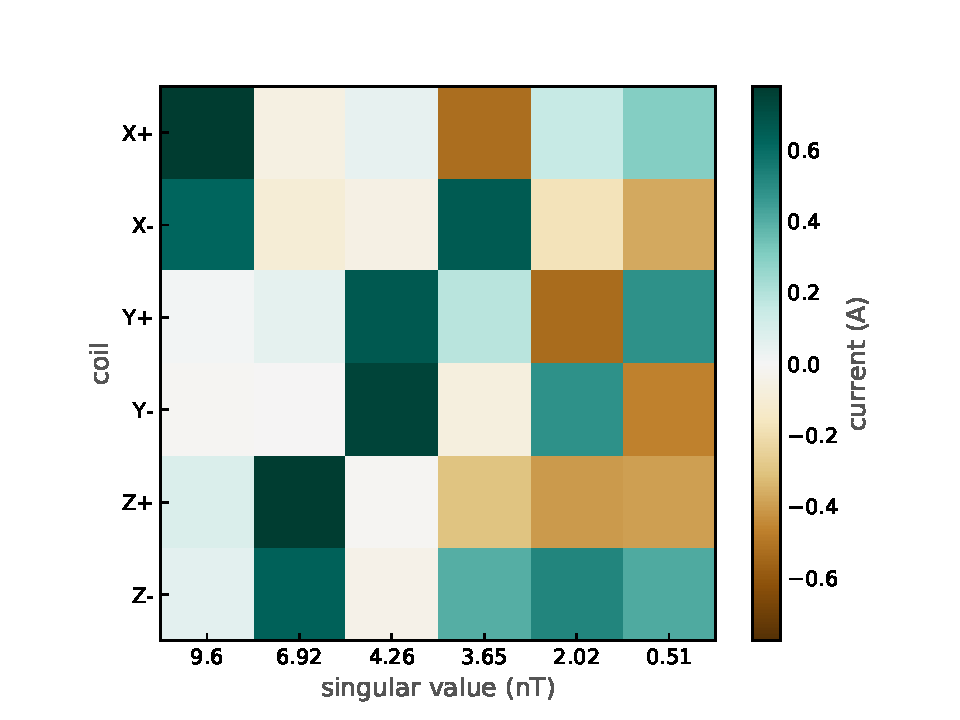
\includegraphics[width=.7\linewidth]{gfx/nEDM_SFC/coil-singular_vectors_of_the_nEDM_SFC_matrix}
  \caption
  [TODO]
  {The coil-singular values of the SFC matrix. Columns correspond to singular combinations of the coils. For each column the corresponding singular value is indicated. See text for details.}
  \label{fig:nEDM_SFC_svd}
\end{figure}

It is to note that the SFC matrix is defined solely by the configuration of the coils and sensors. It follows that care has to be taken already at the design stage to create a system that will be well defined.


\section{Optimising the number of windings in the coils}
Put the plots of the distributions of the currents, juxtapose them with the
ranges of the power supplies.


\section{Visualisation of the data}
The data of the SFC system are difficult to visualise. Mostly because the magnetic field is a three dimensional field in a three dimensional space. It is much easier to explore if they are visualised interactively. Together with a student, Nils Ebeling, we created a visualisation.

Possibility to show the calculated external field!

The program is cross--platform (Windows, OSX, Linux), fully based on open--source softwore. It is written in python and uses the following libraries: Qt4 (cross-platform GUI), pyqtgraph (fast interactive plotting), VTK (3D graphics) and SciPy (data handling).

\begin{figure}[bth]
  \myfloatalign
  \subfloat[Displaying the calculated back external field, the movable yellow cursor chooses the data to be displayed in the 3D view.]{
    \label{fig:nEDM_SFC_visualisation1}
    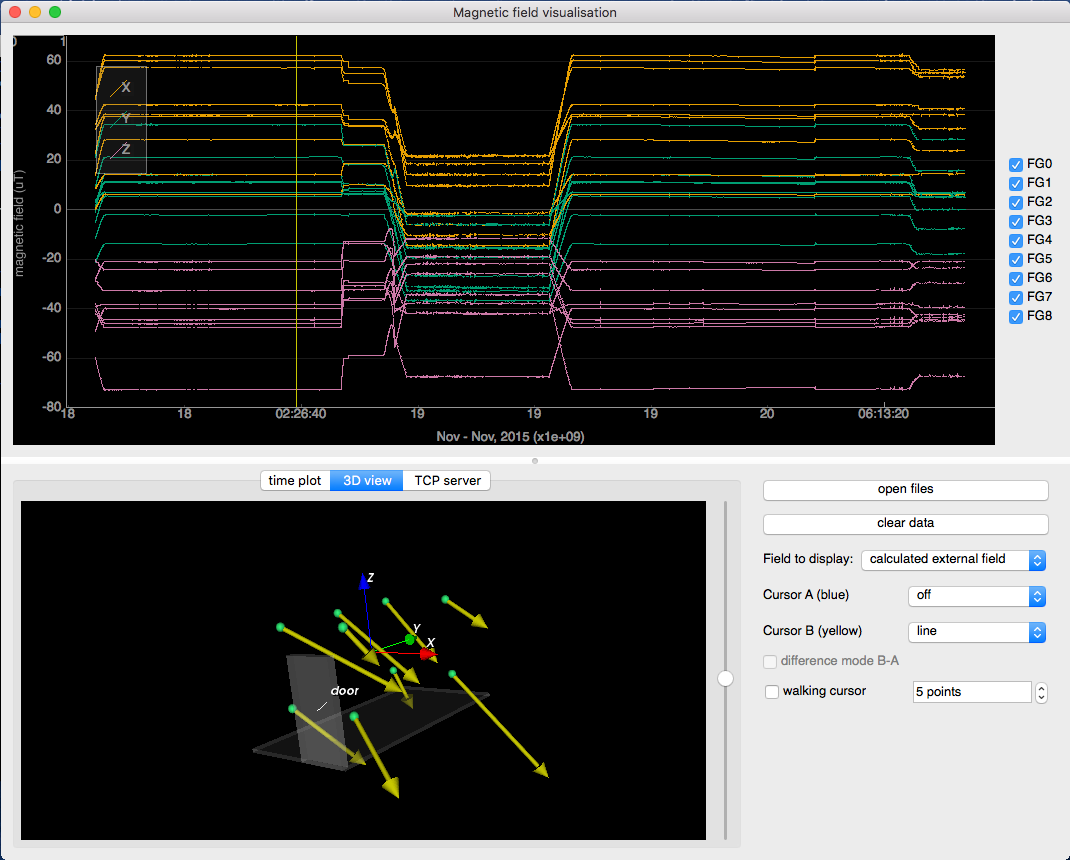
\includegraphics[width=.45\linewidth]{gfx/nEDM_SFC/visualisation/visualisation1}}
  \quad
  \subfloat[Displaying fields at two different times simultaneously, yellow and blue.]{
    \label{fig:nEDM_SFC_visualisation2}
    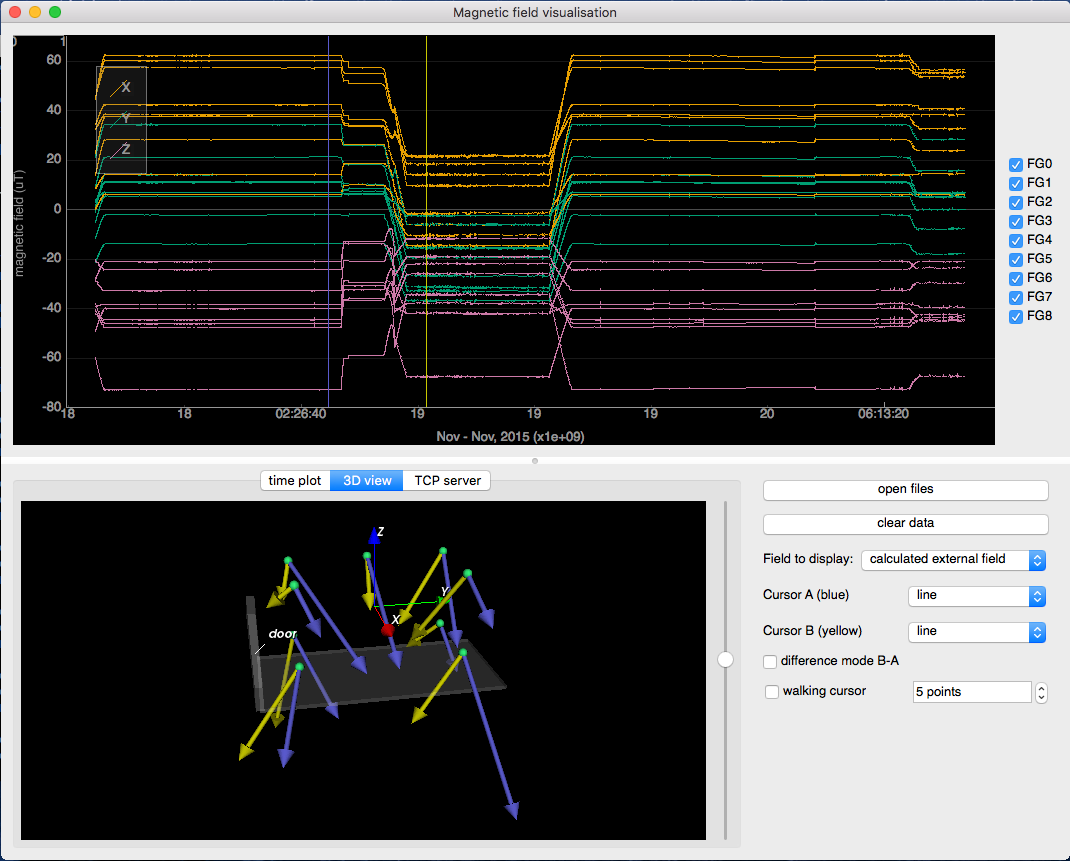
\includegraphics[width=.45\linewidth]{gfx/nEDM_SFC/visualisation/visualisation2}}
  \\
  \subfloat[Displaying a range of data, marked with the yellow cursor, relative to the point marked with the blue cursor. The calculated back external magnetic field is displayed.]{
    \label{fig:nEDM_SFC_visualisation3}
    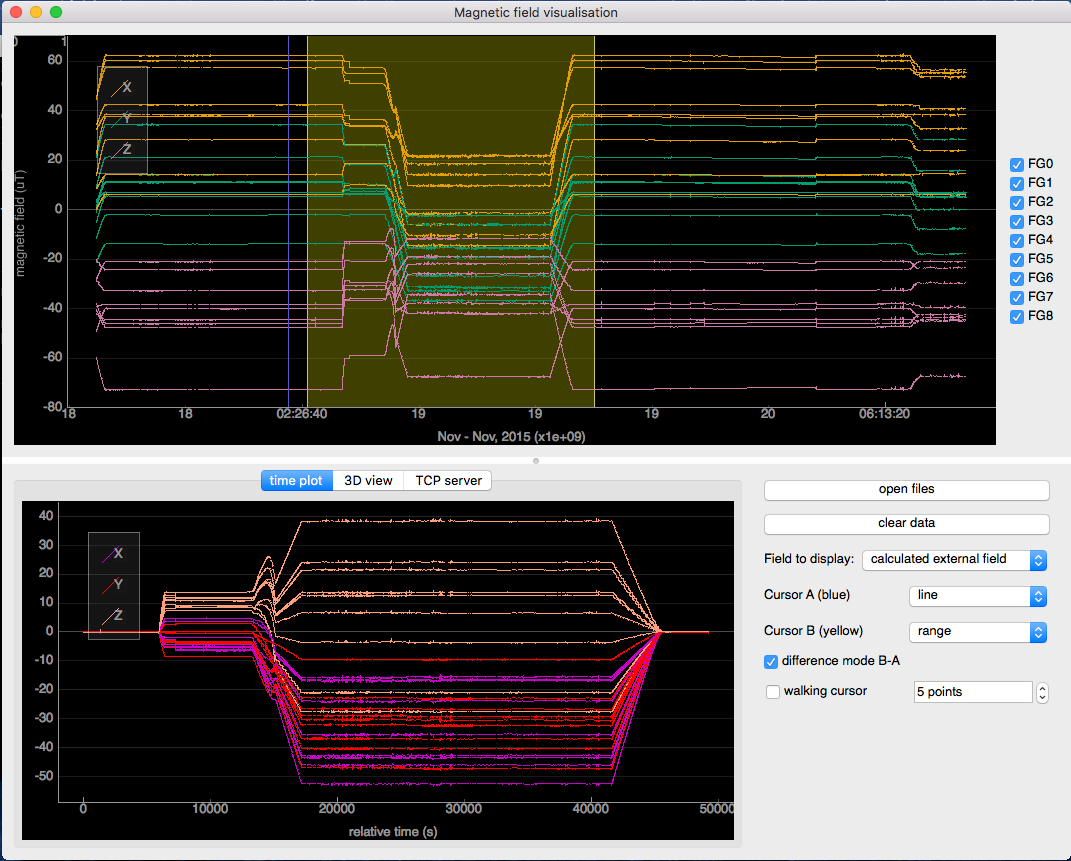
\includegraphics[width=.45\linewidth]{gfx/nEDM_SFC/visualisation/visualisation3}}
  \quad
  \subfloat[Displaying the difference between the external field in two points in geometrical form.]{
    \label{fig:nEDM_SFC_visualisation4}
    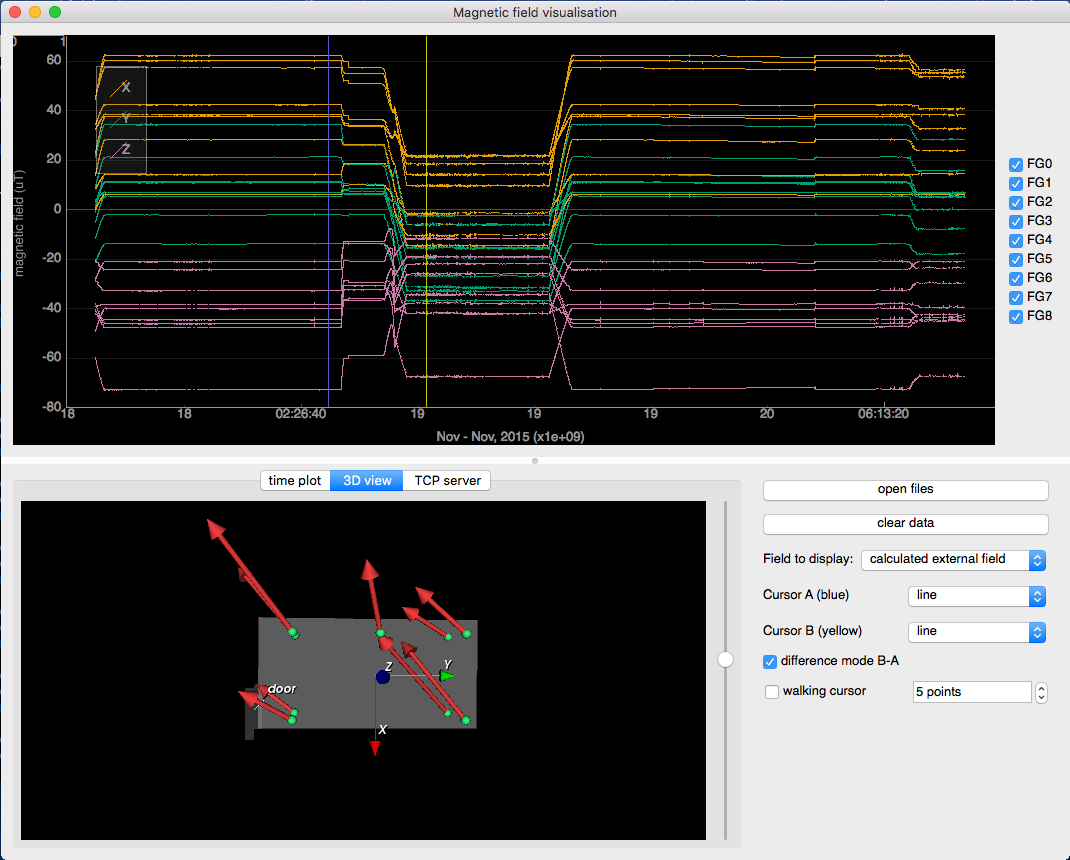
\includegraphics[width=.45\linewidth]{gfx/nEDM_SFC/visualisation/visualisation4}}
  \caption{Different functionalities of the nEDM SFC data visualisation tool.}
\end{figure}

Write here about the program and the tricks used (subtract the value under the cursor) and so on. Also about the 3D representation. Here show how does the field of SULTAN look like, in time and in 3D.

Work of Nils Ebeling.


\section{Performance during SULTAN ramps}
Describe the fancy algorithm and show the results of the data analysis.



\section{Remote magnetometers}
Write the documentation, show a SULTAN ramp as seen by the magnetometers, boast a bit about the automatic deployment, timing accuracy and so on.

Work of Gianluca Janka.

Despite five layers of mu-metal shielding the external magnetic field environment will play an important role in the n2EDM experiment, as it does in the nEDM. One handle on monitoring it are the sensors of the Surrounding Field Compensation system. However, as they are inside the compensation system, and in the direct vicinity of the shield, it is hard to infer about the external sources of magnetic disturbance. Remote magnetometers will be distributed around the experiment site, around 10 meters away.

The primary role of the remote magnetometers system is to measure the magnetic environment around the experiment. Thanks to their spatial distribution it is easy to identify the approximate direction of the source of the disturbance. This is a valuable input for the shifters who may, for example, decide to delay a start of sensitive measurement seeing that a nearby magnet is ramping. In the off-line analysis a reason for an abnormal behavior may be correlated and attributed to a particular external source of magnetic disturbance.

For the 2016 operation a prototype array of 4 remote magnetometers has been set up, each placed approximately 10 meters away from the experiment. In Fig.\,\ref{fig:remote_magnetometers_ui} a ramp of the SULTAN magnet is shown, as seen by the magnetometers. The sensors are based on widely used commercially Inertial Measurement Units (IMU) in form of a chip, which include a magnetometer. The sensitivity of those, about 0.1$\,$µT, is enough for a remote magnetometer. We use an IMU chip on the senseHAT module for a RaspberryPi single-board computer. The two, with appropriate software, form a measurement module, including data transmission. A module has also a power-over-ethernet splitter, so an ethernet cable is the only connection to a module. A photograph of a complete remote magnetometer module is presented in Fig.\,\ref{fig:remote_magnetometers_remote_magnetometer}. All of the hardware is off-the-shelf. The measurements on all modules are synchronous on a $\approx20\,$µs level with the use of precise time protocol (see Fig.\,\ref{fig:remote_magnetometers_timing_measurement}. The data from all magnetometers is aggregated on a single computer (also a RaspberryPi) and transmitted over an optical link to the main DAQ.

\begin{figure}
  \centering
  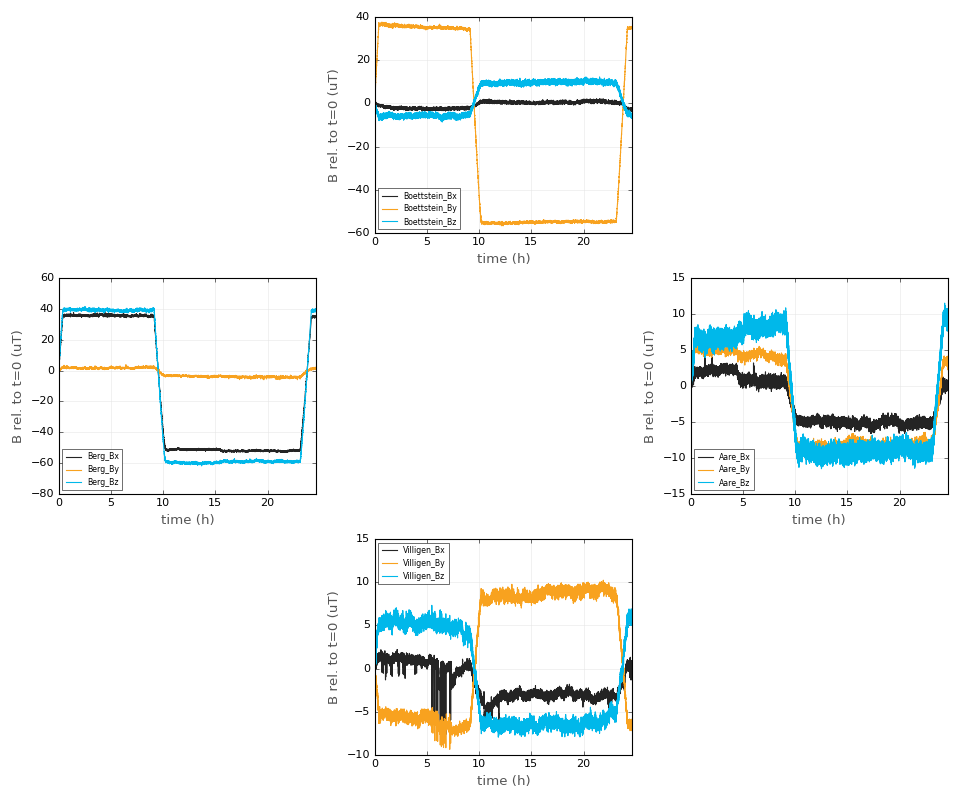
\includegraphics[width=\linewidth]{gfx/nEDM_SFC/ui_plot.png}
  \caption{The up- and down-ramping of the SULTAN magnet seen by the four prototype remote magnetometers. The positions of the plots roughly correspond to the location of the sensors, the experiment being in the middle. For each magnetometer the three components of the magnetic field are plotted, but the orientation is not consistent between plots. The immediate conclusion can be drawn, that the magnet is located in the direction up and left.}
  \label{fig:remote_magnetometers_ui}
\end{figure}

\begin{figure}
  \centering
  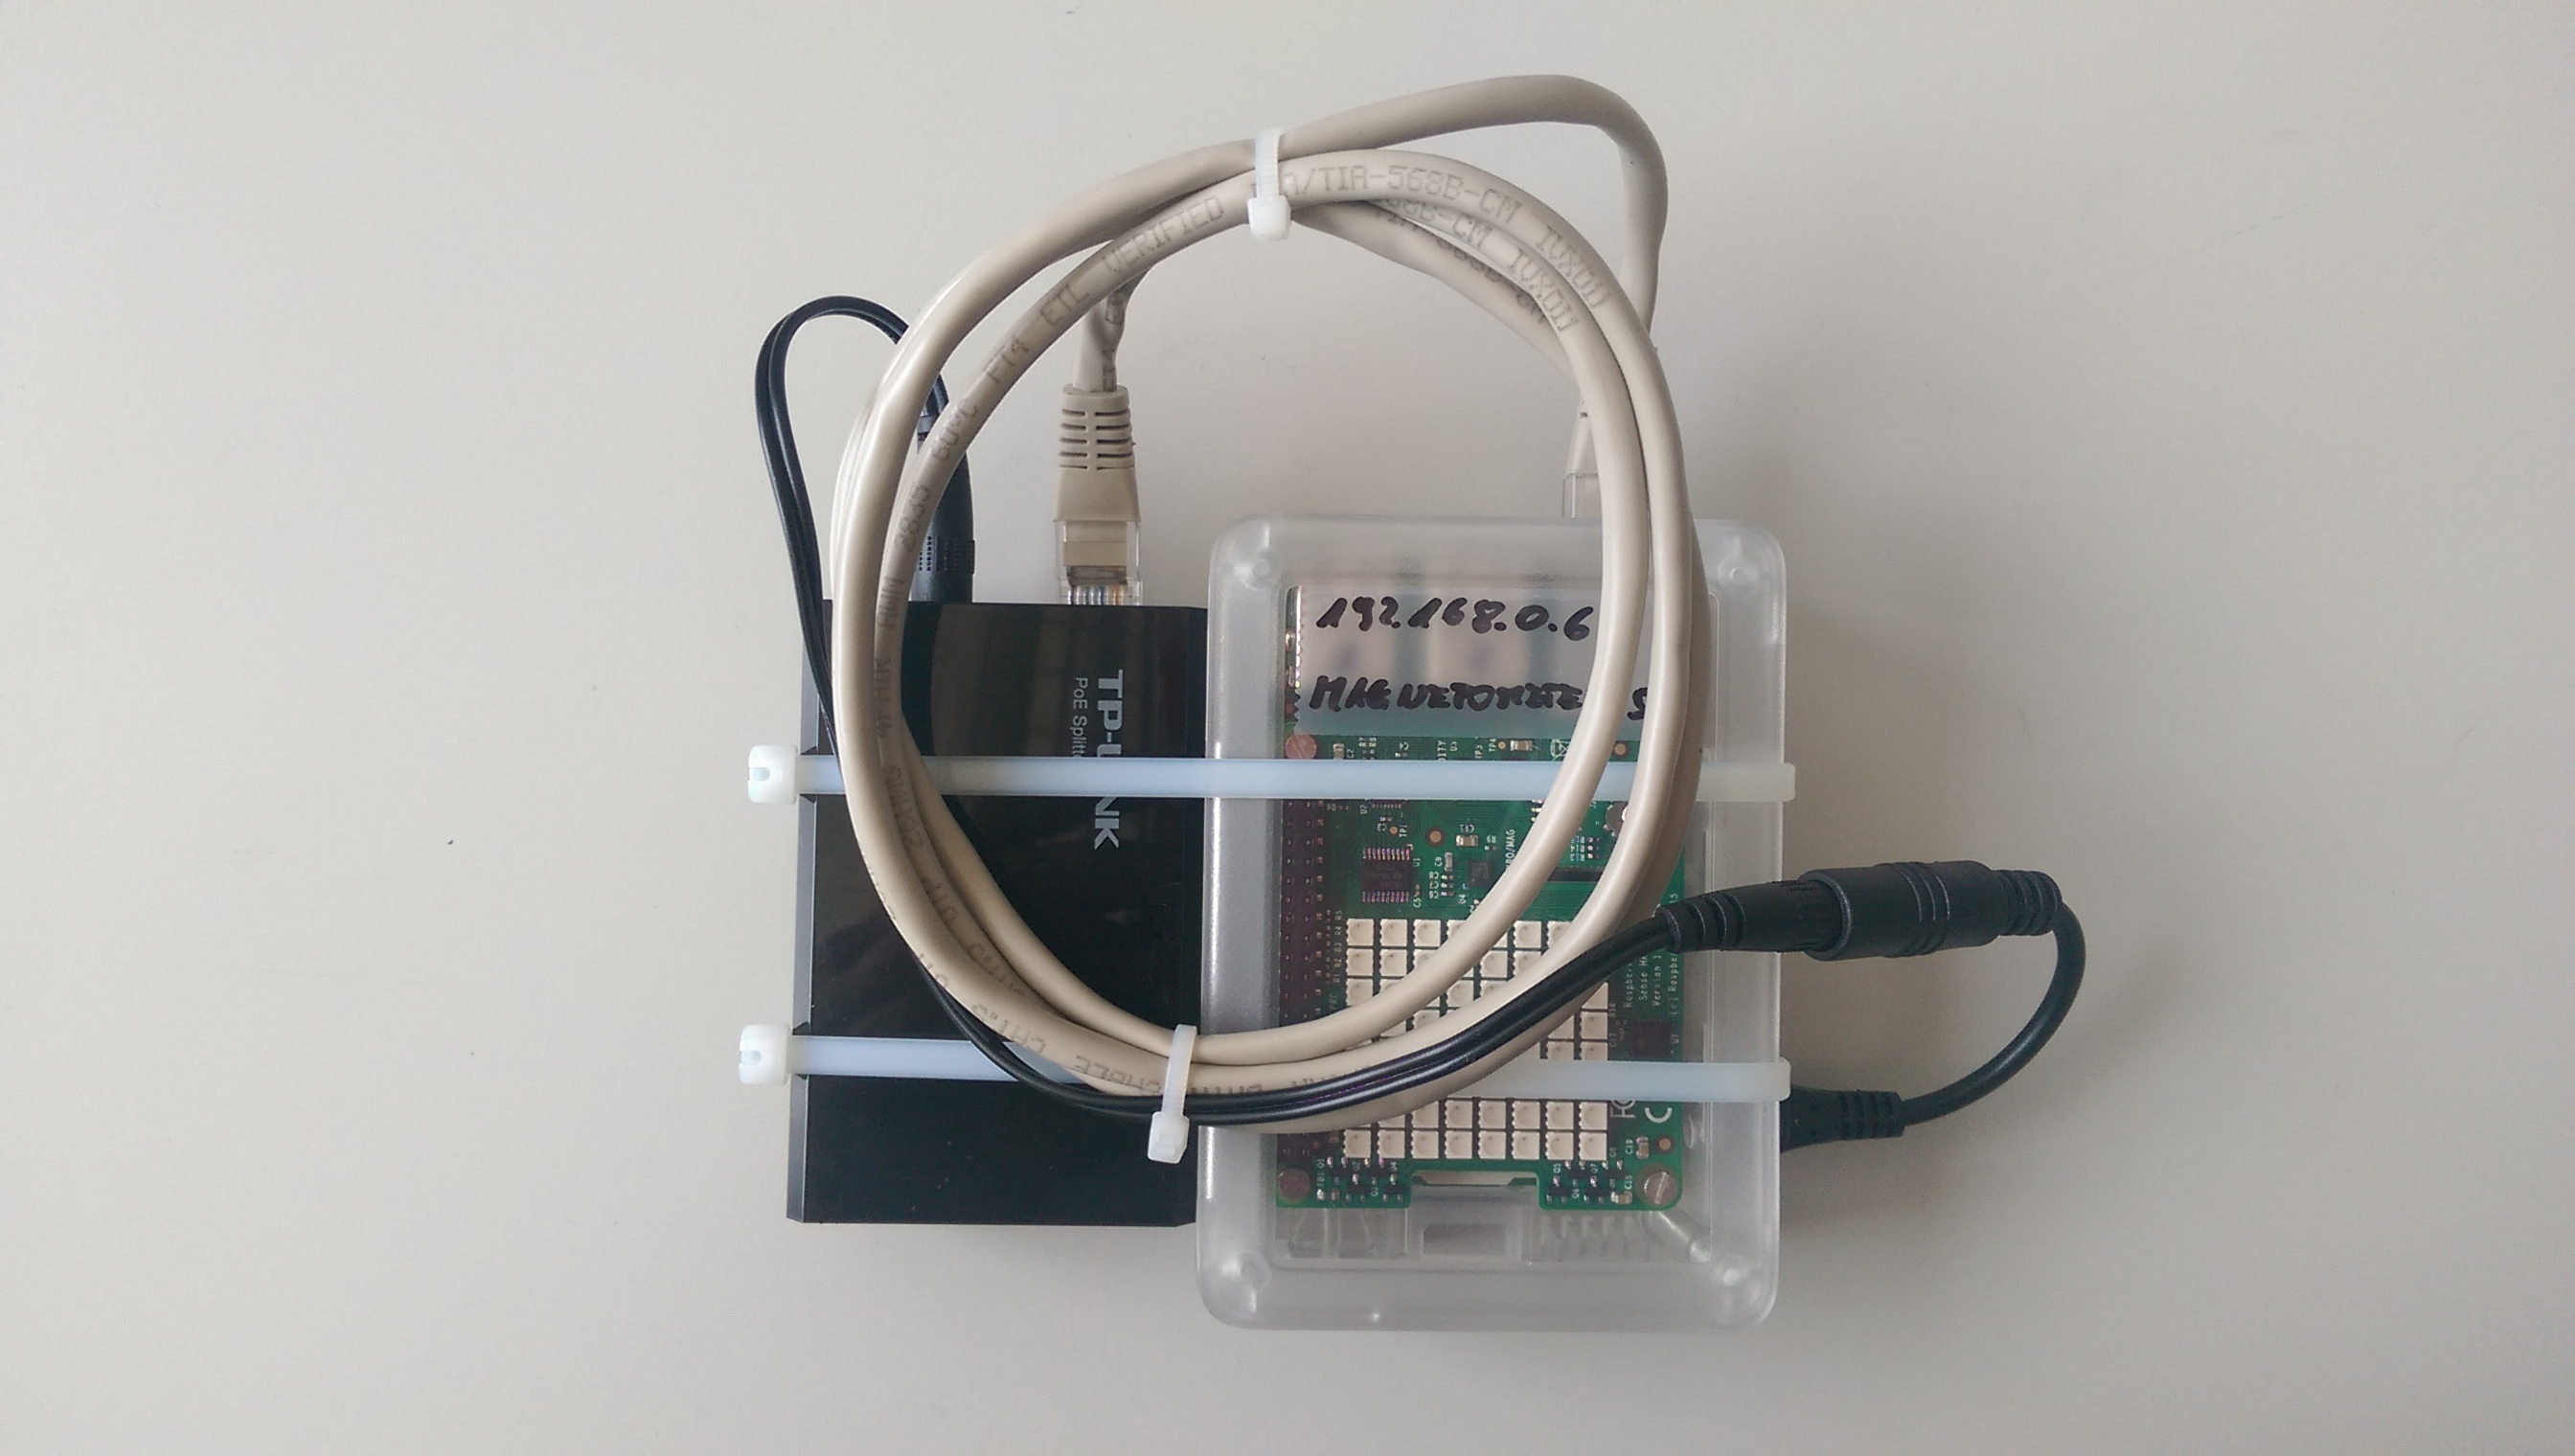
\includegraphics[width=\linewidth]{gfx/nEDM_SFC/remote_magnetometer.jpg}
  \caption{A prototpype remote magnetometer module. On the right is a RaspberryPi single--board computer with a senseHAT module, the latter including a magnetic field sensor. Both are protected by a transparent, commercial enclosure. The black part on the left is a power-over-ethernet splitter (TP-Link TL-PoE10R). The ethernet interface of the whole module, for both data transmission and power, is located on the bottom of the splitter.}
  \label{fig:remote_magnetometers_remote_magnetometer}
\end{figure}

\begin{figure}
  \centering
  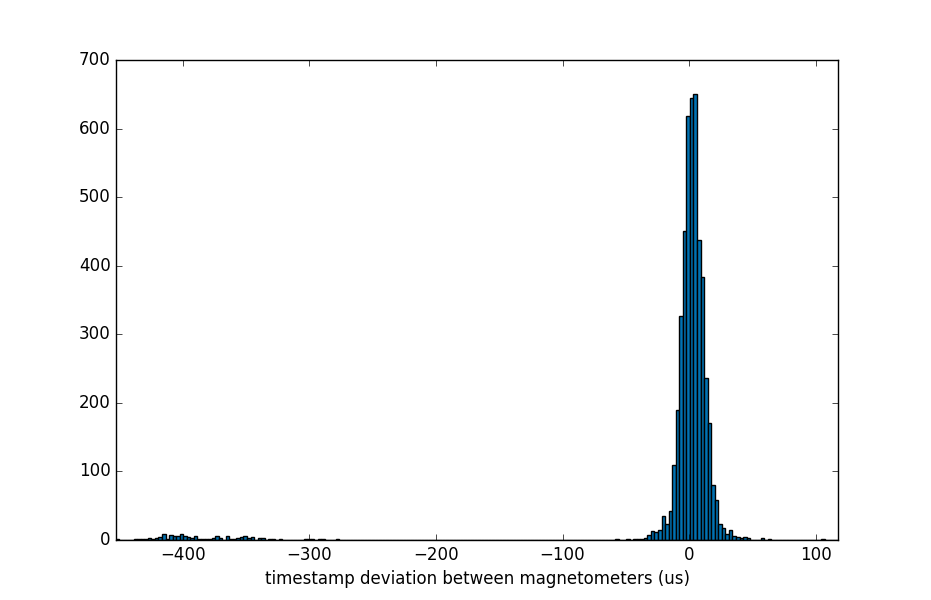
\includegraphics[width=\linewidth]{gfx/nEDM_SFC/timing_measurement.png}
  \caption{The histogram of the the time jitter between remote magnetometers synchronised over precise time protocol. The jitter is on a 20µs level, with rare events at around 400µs.}
  \label{fig:remote_magnetometers_timing_measurement}
\end{figure}

For the n2EDM the remote magnetometers system is mainly going to be scaled to approximately 50 modules, which requires no change in the architecture. Both software and choice of hardware are to be directly transferred from the prototype. Minor work will need to be done in the data transmission front-end to adapt to the n2EDM DAQ scheme. It is planned to additionally design and manufacture custom adapters for mounting the modules in the experimental hall. The projected cost, totalling at around 11$\,$kCHF, is summarized in Table\,\ref{tab:remote_magnetometers_cost}. It workload is estimated to be 36 full-time-equivalent days to complete, not counting the workshop's time for manufacturing the mountings.


\begin{table}
  \centering
  \begin{tabular}{lrrr}
    \toprule
    Item  & Unit Cost & Quantity & Item Cost \\
    %  &  & (CHF) & (CHF) \\
    \midrule
    RaspberryPi model B & 46 & 50 & 2300 \\
    RaspberryPi senseHAT & 46 & 50 & 2300 \\
    8GB SD card & 13 & 50 & 650 \\
    ModMyPi Modular RPi 2 Case & 13 & 50 & 650 \\
    TP-Link TL-PoE10R PoE Splitter & 10 & 50 & 500 \\
    Ethernet cable 30m & $\approx\,$50 & 50 & $\approx\,$2500 \\
    Cisco SG500-52P-K9-G5 PoE Switch & 1468 & 1 & 1468 \\
    Mountings & $\approx\,$20 & 50 & $\approx\,$1000 \\
    \cmidrule{3-4}
    & & Total Cost & $\approx\,$11\,000 \\
    \bottomrule
  \end{tabular}
  \caption{Summary of the cost of the remote magnetometers system for n2EDM. excluding the production of the mountings. All prices in Swiss Francs.}
  \label{tab:remote_magnetometers_cost}
\end{table}
